\documentclass{article}

\usepackage[twocolumn,landscape,a4paper,margin=15mm,columnsep=30mm]{geometry}
\usepackage{graphicx}
\usepackage{parskip}
\usepackage{color}
\usepackage{PTSansNarrow} 
\usepackage[T1]{fontenc}
\usepackage[dutch]{babel}
\usepackage{array}
\renewcommand\familydefault\sfdefault

\pagestyle{empty}

\definecolor{myred}{rgb}{0.92,0.11,0.15} % #eb1c26
\definecolor{mygray}{rgb}{0.82,0.82,0.82}

\newenvironment{myquote}
{%
  \begin{quote}
  \begin{picture}(0,0)\put(-20,-34){\fontsize{2cm}{1em}\selectfont\bf\color{mygray}``}\end{picture}
  \raggedright
  \setlength\parindent{1.5ex}
}{%
  \end{quote}
}

\newcommand\largeblack[2]{{\fontsize{#1}{1em}\selectfont\bf#2}\par}

\newcommand\myhline{\textcolor{myred}{\rule{\columnwidth}{6pt}}}
\newcommand\mysep{\textcolor{mygray}{\hfill$\bullet$\hfill}}
\newcommand\mymega[1]{{\fontsize{1.15cm}{1em}\selectfont\bf#1}\par}
\newcommand\myhuge[1]{\textcolor{red}{\Huge\bf#1}\par}
\newcommand\mylarge[1]{\textcolor{red}{\Large\bf#1}\par}
\newcommand\mybox[1]{\colorbox{myred}{\parbox{\columnwidth}{\centering\parbox{.95\columnwidth}{\rule{0pt}{13pt}\color{white}\large\bf#1\rule[-7pt]{0pt}{0pt}}}}}

\newcommand\mytitle[1]{%
  \renewcommand\arraystretch{2}
  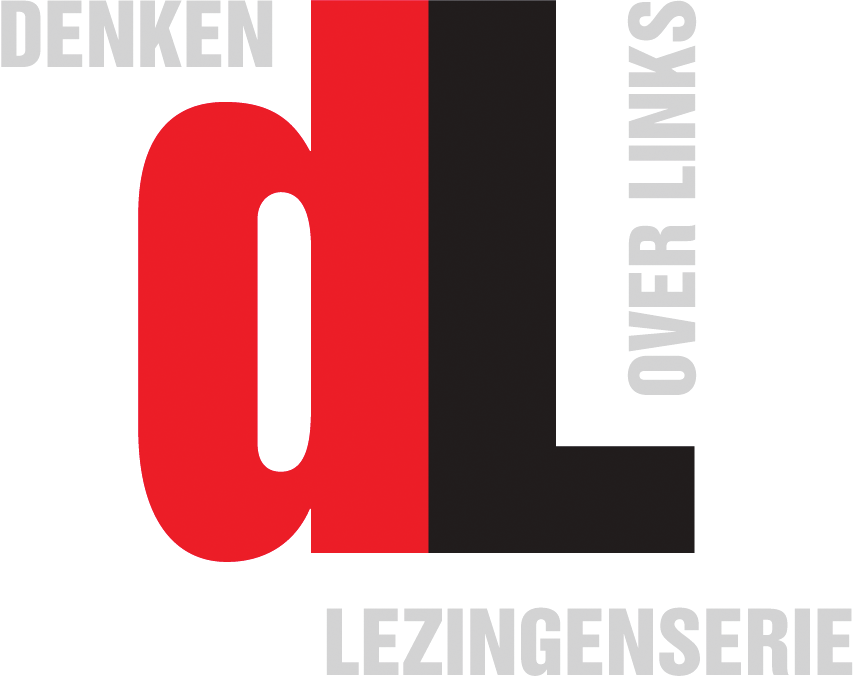
\includegraphics[width=.6\columnwidth]{dol_logo.png}\hfill\begin{tabular}[b]{@{}>{\color{red}\Huge\bf}r@{}}#1\end{tabular}\par
  \myhline \\
  {\bf Gaffelstraat 61B \mysep Toegang gratis \mysep Inloop: 19:30 uur \mysep Start: 20:00 uur \mysep Eind: 22:00 uur} \\
  \myhline
  \par\vspace{7mm}\par
}
 % packages, settings, functions

\begin{document}

\mytitle{.3\columnwidth}{Europa: waarheen, waarvoor?}

\mymega{DONDERDAG 13 JUNI}

\vfill

\textbf{Onder het motto `denken over links' biedt de SP Rotterdam in haar
nieuwe onderkomen aan de Gaffelstraat een podium voor inspirerende sprekers
over diverse thema's als samenleven in de stad, actief burgerschap, economie en
Europa. Een maandelijkse lezingenserie waarin het denken over hedendaagse
sociale vraagstukken wordt geprikkeld en gescherpt.}

\vfill

\mylarge{Sprekers}

\vfill

\textbf{\large Willem Bos}
\begin{quote}
  Woordvoerder Comit\'e Ander Europa
\end{quote}

\vfill

\textbf{\large Kayleigh van Oorschot}
\begin{quote}
  Onderzoeker bij de Nederlandse School voor Openbaar Bestuur. Zij haalde haar
  master European Studies: Ideas and Identities aan de London School of
  Economics and Political Science.
\end{quote}

\vfill

\mybox{`Denken over links', een maandelijkse lezingenserie in het SP-pand aan
de Gaffelstraat. Doe mee, denk mee! Iedereen is welkom.}

\newpage

\myhuge{Europa: waarheen, waarvoor?}

\vfill

\textbf{Het is dit jaar pas twintig jaar geleden dat in november 1993 in
Maastricht de Europese Unie werd ingesteld. Een relatief korte periode, waarin
veel is veranderd. Zo is het aantal lidstaten meer dan verdubbeld van 12 tot
27. In 17 daarvan is de euro ingevoerd. Een verregaande herziening de
organisatie werd in 2005 per referendum verworpen, om in 2009 alsnog aangenomen
te worden. Veel voorheen nationale besluitvorming is ``verschoven naar
Europa''. En in 2012 ontving de EU de Nobelprijs voor de Vrede.}

\vfill

Illustraties van een razendsnelle ontwikkeling, en voeding aan een doorlopend
en fel debat over de toekomst van het project. Tegenover elkaar staan de
eurofielen, ook wel federalisten, die Europa economische voorspoed en
eeuwigdurende vrede toedichten. En de eurosceptici, die wijzen op het
ondemocratische gehalte en de liefde voor het grootbedrijf. Ondertussen zucht
het continent onder de grootste economische depressie sinds de crisisjaren 30,
en wijzen alle vingers naar de EU als oorzaak en oplossing. De controverse als
belangrijkste kenmerk van de unie.

\vfill

\mylarge{Met onze gasten schijnen we licht in deze duisternis.}

\vfill

\textbf{Willem Bos} was organisator van de Grondwet NEE campagne in 2005. Hij is
woordvoerder van het Comit\'e Ander Europa, lid van de SAP en redacteur van
grenzeloos, waarin hij met regelmaat kritische opiniestukken schrijft.
\begin{myquote}
  Hebben we in de Europese Unie te maken met een democratisch tekort dat op
  termijn weggewerkt kan worden of is dat gebrek aan democratie juist een
  wezenskenmerk van de huidige Unie? Als we het functioneren van Europa de
  afgelopen decennia bezien, kunnen we niet anders dan het laatste concluderen.
\end{myquote}
{\footnotesize Uit: Europa en Democratie: Best wel een goed idee! Brochure 2012}

\vfill

\textbf{Kayleigh van Oorschot} haalde vorig jaar haar master European Studies: Ideas and
Identities aan de London School of Economics and Political Science. Ze werkt nu
als onderzoeker bij de Nederlandse School voor Openbaar Bestuur.
\begin{myquote}
  Als we onze samenleving de ruimte willen geven om zich te ontwikkelen, om te
  verbeteren en vooruit te bewegen en als we, met de woorden van Frans
  Timmermans, 'uit de crisis willen groeien', moeten ook wij weer utopisch gaan
  denken.
\end{myquote}
{\footnotesize Uit: Pleidooi voor de utopie. Groene Amsterdammer, 25 maart 2013}

\vfill

Nieuwsgierig? Kom langs en debateer met ons mee op 13 juni op de Gaffelstraat.
Aanvang 20:00, deur open 19:30. De toegang is gratis.

\myhline

\end{document}
